\documentclass[11pt, twoside]{article} %iniciación del documento de tipo artículo, con tamaño de letra 11pt.
\usepackage[a4paper,total={6in, 8in},left=25mm, asymmetric]{geometry} %Cambio en los bordes y margenes del documento

\usepackage{fancyhdr} %Paquete para organizar y añadir header con los nombres

\usepackage{amsmath}

\usepackage[spanish,es-tabla,es-nodecimaldot]{babel}
\usepackage{tabularx}
\usepackage{booktabs}

\usepackage{caption}

\usepackage{graphicx}
\usepackage[hidelinks]{hyperref}
\usepackage{macro}

\fancypagestyle{main}{
    \fancyhf{}
    \fancyhead[L]{\thepage}
    \fancyhead[RO]{ZhuoZhuo L.}
    \renewcommand{\headrulewidth}{.4pt}
    \setlength{\headheight}{52pt}
}

\pagestyle{empty}

\begin{document}

\begin{figure}[h!]
    \minipage{0.87\textwidth}
	
\includegraphics[width=3cm]{Icons/ugr.jpg}
	\endminipage
    \minipage{0.87\textwidth}
	
\includegraphics[height = 2.5cm, width=3cm]{Icons/facultad_ciencias.png}
	\endminipage
	%%\vspace{-1cm}
\end{figure}

\vspace{0.3cm}

\begin{center}
    \Huge \textbf{Física Computacional}\\
    		\vspace{0.4cm}
    \LARGE \textbf{Voluntario 1:}  
    Simulación con dinámica molecular de un gas con un potencial de Lennard-Jones
\end{center}

\vspace{1cm}

\vspace{1cm}

\begin{center}
    \large \textbf{Resumen}\\
    		\vspace{0.2cm}
    \normalsize
    En este informe tenemos como objetivo estudiar el comportamiento de un sistema que
    interactuan mediante un potencial de Lennar-Jones. Princialmente se estudiará 
    la distribución de velocidades de las partículas, la ecuación de estado y la 
    transición de fase.

\end{center}

\vspace{1cm}

\begin{flushright}
    \large Zhuo Zhuo Liu 
    \\
    \vspace{0.4cm}
    \textbf{Grado en Física}
\end{flushright}

\newpage

\setcounter{page}{0}
\tableofcontents
\newpage

\pagestyle{main}

\section{Introducción}

El potencial de Lennard-Jones es un modelo que describe la interacción entre dos
partículas neutras, y es ampliamente utilizado en la simulación de sistemas
de partículas, debido a su simpleza, sin embargo sigue siendo capaz de describir
las interacciones de una manera realista.

\section{Planteamiento del problema}

Para poder simular el sistema, se ha de tener en cuenta muchas cosas, como las 
condiciones iniciales o las condiciones de contorno, las cuales se describirán a 
continuación, junto a otros problemas a tener en cuenta.

\subsection{Condiciones iniciales}
Comenzando por las condiciones iniciales del sistema, al introducir estas, 
debemos de tener cuidado de no colocar 2 partículas muy cercas entre ellas, ya que 
puede provocar que las partículas adquieran mucha velocidad, colapsando el sistema.

Para ello consideramos una cuadrícula separada por una distancia $2\sigma$ en ambos 
ejes, y permitimos que las partículas se desplace una distancia aleatoria entre 0 y 1
de dicha posición. De esta manera se asegura que la distancia mínima posible inicialmente
sea de $1\sigma$. 
\subsection{Condiciones de contorno}

Para introducir la condición de contorno bidimensional periódica empleamos 
2 funciones, una para la posición de las partículas, y la otra para la 
distancia entre partículas. Pero ambos seguirán la misma lógica.

Comenzando para la posición de las partículas, se tiene que si una partícula en su
nueva posición tiene una coordenada mayor que $L$ o menor que 0, entonces se le 
restará o sumará $L$ a dicha coordenada dependiendo del caso. 

Mientras que para la distancia entre partículas, se tiene que si la distancia entre
partículas en una de las coordenadas es mayor que $L/2$, entonces se le restará 
$L$ a la distancia. Y aplicando lo mismo al caso contrario, cuando la distancia es
menor que $-L/2$.

Notar que se ha tenido que diferenciar en 2 funciones muy similares, pero con diferentes
condiciones, ya que el sistema no está centrado en 0. Si se hubiera centrado en 0, 
ambas funciones serían iguales.

Una vez tenida estas condiciones, ya podemos calcular la distancia entre partículas,
estas distancias será importantes tanto para calcular las fuerzas de interacción, como 
la energía potencial del sistema. Guardaremos estas distancias o mejor dicho los vectores que las unen en una matriz 
de dimensiones $N\times N\times 2$, donde $N$ es el número de partículas, y 2 indica
las dimensiones del espacio. El cálculo de estas distancias es sencillo, siendo la
resta entre las posiciones de las partículas. 

Podemos reducir el número de cálculos al notar que la matriz es antisimétrica, entonces el 
elemento $R_{ij}$ es igual a $-R_{ji}$, por lo que solo necesitamos calcular menos de 
la mitad de la matriz, y asignar el valor correspondiente a los otros elementos.

\subsection{Potencial Lennard-Jones}

Una vez tenido las funciones para imponer la condición de contorno y el cálculo de 
las distancias entre partículas, podemos calcular la fuerza de interacción entre 
partículas por el potencial de Lennard-Jones.

\begin{equation}
    V(R) = 4\epsilon\brackets{\parenthesis{\frac{\sigma}{R}}^{12}-
        \parenthesis{\frac{\sigma}{R}}^{12}},
    \label{eq:Lennard_Jones_potential}
\end{equation}
donde se ha usado $R$ en lugar de $r$, para coincidir en la notación empleada en 
el código.

\vspace{3mm}

Entonces la fuerza de interacción entre las partículas viene dado por:

\begin{equation}
    \vec{F}(\vec{R}) =  - 4\epsilon\brackets{6\parenthesis{\frac{\sigma}{R}}^{5}-
    12\parenthesis{\frac{\sigma}{R}}^{11}}
\end{equation}

Para calcular la aceleración de la partícula, se suma la fuerza de interacción con
todas las demás las partículas, y se divide por la masa. Implementando en todo esto en la función que te devuelve la aceleración del sistema
en función de la posición de las partículas.

Por último solo queda añadir una función que nos permita calcular la nueva posición
de las partículas, y la nueva velocidad de las partículas. Para ello emplearemos el
algoritmo de Verlet. 

\subsection{Unidades empleadas}

Se ha empleado el sistema de unidades reducidas, donde la energía y la distancia se 
expresan en función de una cantidad característica, en este caso $\epsilon$ y $\sigma$. 
De modo que para las diferentes magnitudes se tiene:
\begin{itemize}
    \item Longitud: $r^* = \frac{r}{\sigma}$
    \item Energía: $U^* = \frac{U}{\epsilon}$
    \item Temperatura: $T^* = \frac{k_B T}{\epsilon}$
    \item Tiempo: $t^* = t \sqrt{\frac{\epsilon}{m\sigma^2}}$
    \item presion: $P^* = \frac{P\sigma^3}{\epsilon}$
\end{itemize}
donde se ha empleado el simbolo $*$ para indicar que la magnitud que está en unidades 
reducidas, mientras que si no lo tiene se encuentra en unidades del sistema 
internacional. 

Salvo que se indique lo contrario, se supondrá que los valores mencionados en este
informe se encuentran en unidades reducidas.

\subsection{Cálculo de presión}

Para obtener la ecuación de estado, es necesario calcular la presión del sistema. 
En este caso el sistema no tiene paredes rígidas, sino una condición de contorno 
periódica, sin embargo esto no afecta al cálculo de la presión, ya que la presión 
depende del momento transferido. De modo que se supondrá que si una partícula cruza
por las paredes del sistema, el doble del momento con la que lo hace será transferido 
a la pared. Permitiendo calcular el momento total transferido, la fuerza por lo tanto
sería el momento total transferido dividido por el tiempo considerado. 

Por último, la presión se obtiene dividiendo la fuerza por el área, pero en este caso
el sistema es bidimensional, de modo que la presión se obtiene dividiendo la fuerza
por la longitud de la caja.

Una última consideración, solo se ha de empezar a calcular la presión una vez que el
sistema se haya relajado, incluir el periodo de tiempo anterior de ello puede producir
resultados incorrectos. Este mismo razonamiento se puede aplicar para el cálculo de
la temperatura.

\newpage

\section{Análisis de Resultados}

\subsection{Comparación con la distribución de Maxwell-Boltzmann}

Partiendo de las condiciones iniciales propuestas (20 átomos de Argón en una caja 
de $L=10$, distribuida aleatoriamente, y velocidades de módulo 1 con dirección aleatoria), se ha simulado el
experimento durante un tiempo $t = 50$, con un paso del tiempo 
$\Delta t = 0.002$. La evolución del sistema puede visualizarse en formato gif, 
en el propio repositorio ()

Representando la evolución de la energía cinética, potencial y total del sistema
a lo largo del tiempo, se obtiene la figura \ref{fig:energias}.

\begin{figure}[h!]
    \centering
    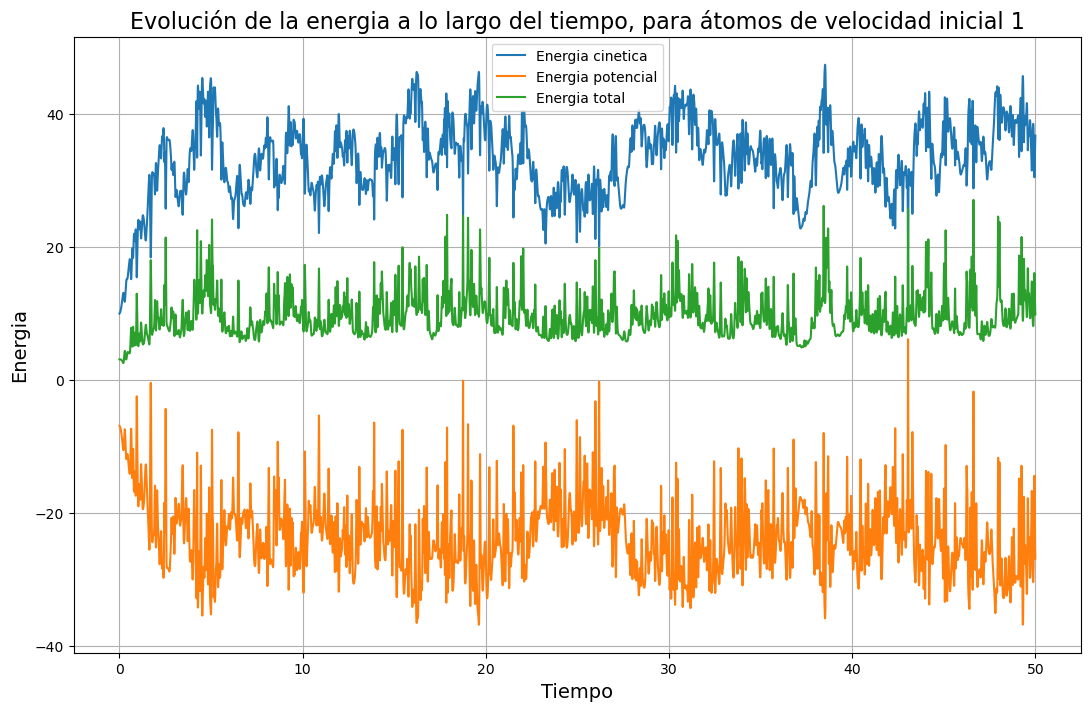
\includegraphics[width=0.9\textwidth]{plots/apartado_1_energia_1.png}
    \caption{Evolución de las energías del sistema}
    \label{fig:energias}
\end{figure}

Se observa como inicialmente la energía cinética aumenta rápidamente, mientras que
la potencial disminuye al mismo ritmo hasta llegar a un punto donde el promedio de 
tanto la energía cinética como la potencial se estabiliza, indicando la relajación 
del sistema, esto ocurre alrededor de $t=10$. Sin embargo para estar seguro, en las 
simulaciones donde la relajación es importante, se esperará un tiempo mayor, $t=20$.

La temperatura se puede obtener por el teorema de equipartición:

\begin{equation}
    k_B T = \frac{m}{2}\langle v_x^2 + v_y^2 \rangle,
\end{equation}
donde se ha considerando que $k_B =1$, y $m=1$.

La temperatura obtenida dependerá de la configuración inicial del sistema, 
principalmente de la distribución inicial de partículas, al ser esta aleatoria,
la temperatura obtenida oscilará, incluso para la misma velocidad inicial. 
La temperatura obtenida será indicado en el título de las figuras.

\begin{figure}[h!]
    \centering
    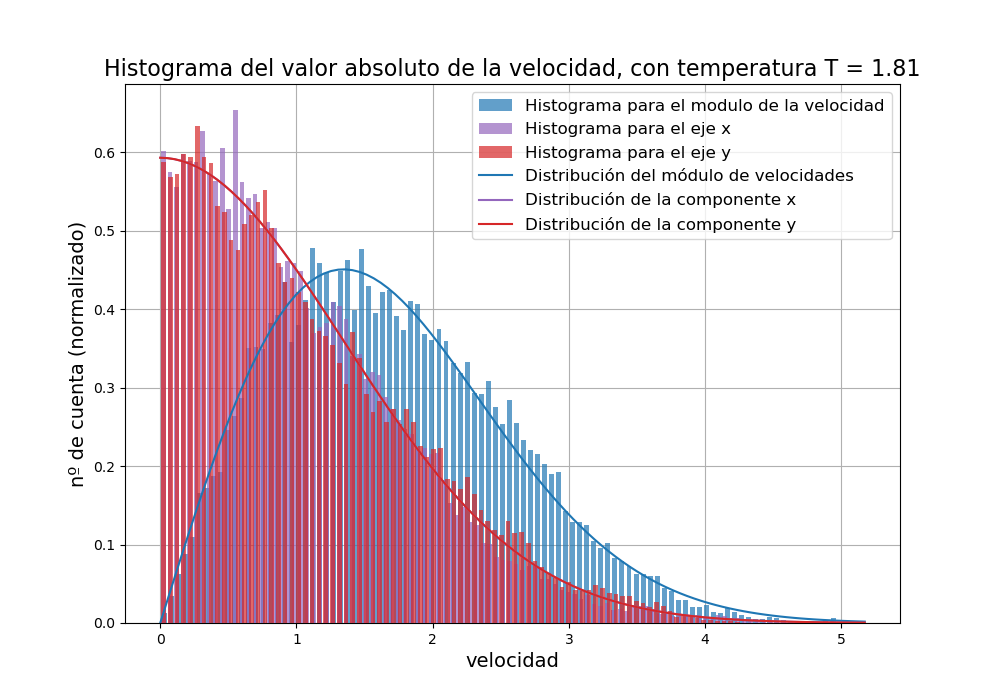
\includegraphics[width=0.9\textwidth]{plots/histograma_velocidad_1.png}
    \caption{Representación del histograma de velocidades para $v, v_x, v_y$ en valor
    absoluto, comparado con las distribuciones de Maxwell-Boltzmann correspondientes. 
    Para velocidad inicial $v=1$, distribuida uniformemente en todas las direcciones.}
    \label{fig:histograma_velocidad_1}
\end{figure}

Comparando la distribución de velocidades antes y después de la relajación con la 
de Maxwell-Boltzmann. Inicialmente todas las partículas tienen la misma velocidad
($v=1$), por lo que la distribución de velocidades es una delta de Dirác. Mientras 
que después de la relajación, la distribución de velocidades se asemeja a la de
Maxwell-Boltzmann, como se observa en la figura \ref{fig:histograma_velocidad_1}.

Este comportamiento se verifica para otras configuraciones iniciales, repitiendo la 
misma experiencia, pero con velocidades únicamente en el eje $x$, de módulo distribuido
uniformemente entre 0 y 1. Se obtiene la figura \ref{fig:apartado_2_energia_x} y 
\ref{fig:histograma_velocidad_x}, indicando la evolución de las energías y la distribución
de velocidades respectivamente.

Empezando por las energías se observa el mismo comportamiento explicado anteriormente, una 
subida inicial hasta llegar a la relajación para la energía cinética, y una bajada hasta 
llegar a la relajación para la energía potencial. Luego para la distribución de velocidades,
se observa que se asemeja a la de Maxwell-Boltzmann, y de manera casi idéntica a la 
figura \ref{fig:histograma_velocidad_1}. De modo que una vez llegado a la relajación,
ambos sistemas son indistinguibles.


\begin{figure}[h!]
    \centering
    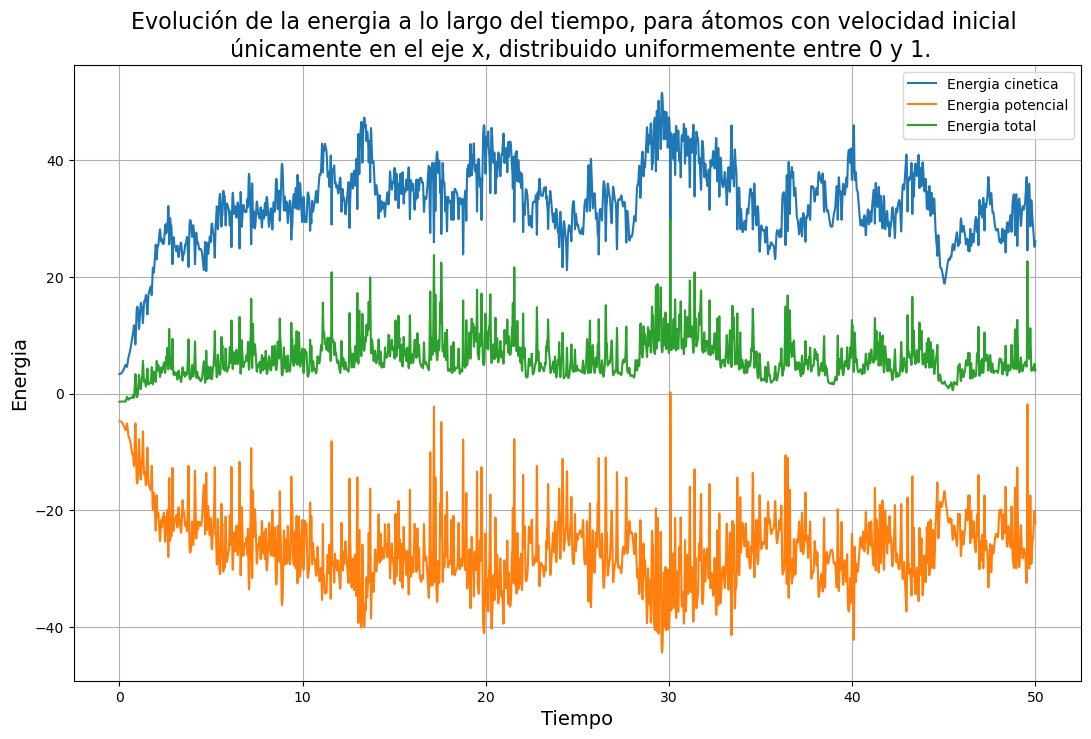
\includegraphics[width=0.8\textwidth]{plots/apartado_2_energia_x.png}
    \caption{Evolución de las energías del sistema, para velocidad inicial distribuida 
    uniformemente entre 0 y 1, solo en el eje $x$.}
    \label{fig:apartado_2_energia_x}
\end{figure}

\begin{figure}[h!]
    \centering
    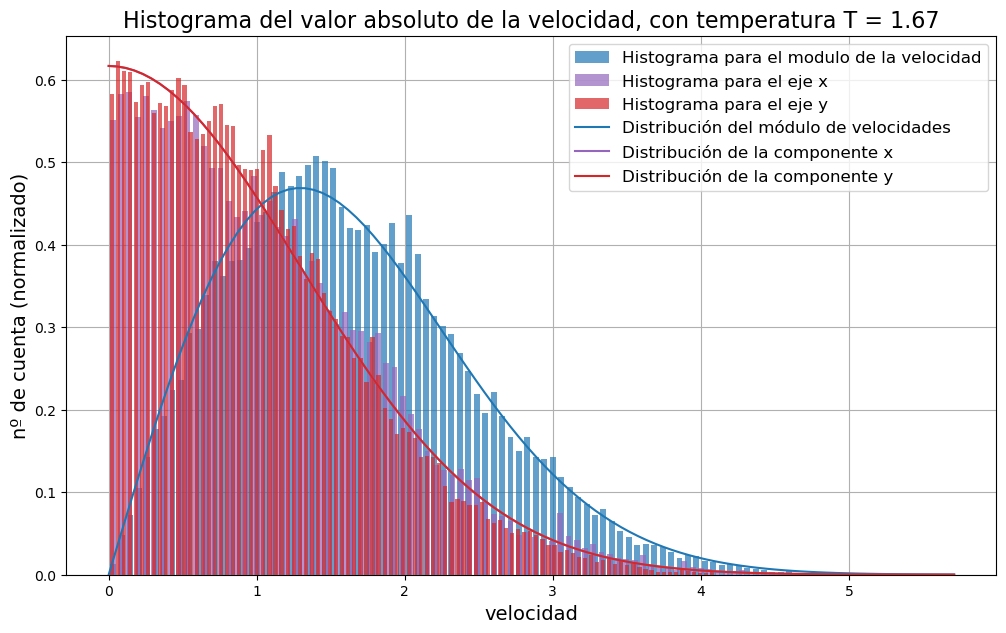
\includegraphics[width=0.8\textwidth]{plots/histograma_velocidad_x.png}
    \caption{Representación del histograma de velocidades para $v, v_x, v_y$ en valor
    absoluto, comparado con las distribuciones de Maxwell-Boltzmann correspondientes. 
    Para velocidad inicial distribuida uniformemente entre 0 y 1, solo en el eje $x$.}
    \label{fig:histograma_velocidad_x}
\end{figure}

\newpage

\subsection{Ecuación de estado}
Considerando un sistema de 16 partículas en una caja de $L=4$, se ha simulado el
experimento durante un tiempo $t=50$, con un paso del tiempo $\Delta t = 0.002$.
En este caso al reducir el tamaño del sistema, se ha tenido que modificar las condiciones
iniciales, para garantizar la estabilidad del sistema, también se ha quitado el carácter
aleatorio de las posiciones iniciales, para poder realizar mejores comparaciones entre 
las diferentes temperaturas.

Tras calcular la presión alcanzada por el sistema, a diferentes temperaturas (para ello
se ha planteado diferentes velocidades iniciales $v = 0, 1, 2, 3, 4$), se obtiene la 
figura \ref{fig:ecuacion_estado}.

\begin{figure}[h!]
    \centering
    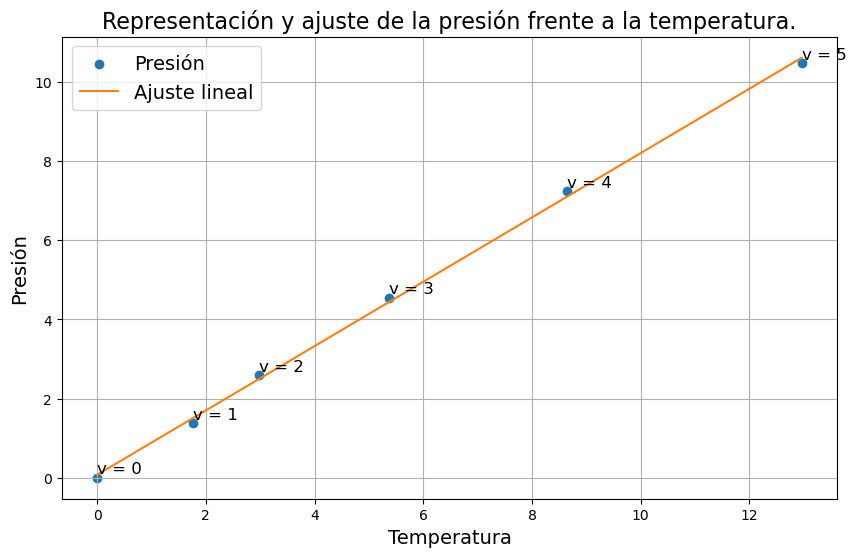
\includegraphics[width=0.9\textwidth]{plots/ajuste_presion.png}
    \caption{Representación de la presión en función de la temperatura, para el sistema
    indicado en este apartado, junto al ajuste lineal realizado entre ambas magnitudes.}
    \label{fig:ecuacion_estado}
\end{figure}

Se ha realizado un ajuste lineal a los datos obtenidos, para obtener la ecuación de
estado del sistema:

\begin{equation}
    P = 0.812 T + 0.076, \text{ con } R^2 = 0.999
\end{equation}


\subsection{Transición de fase sólido-líquido}
Para estudiar la transición de fase sólido-líquido, primero estudiaremos el estado
sólido, para ello se ha empleado un sistema de 16 partículas en una caja de 
$L=4$, con condiciones iniciales de una red cuadrada y en reposo. La idea es ver 
que el sistema evoluciona hasta un estado de equilibrio, donde se dispondrán 
en una estructura triangular.


De hecho este comportamiento se verifica para otras configuraciones iniciales, 
siempre que la temperatura del sistema sea lo suficientemente baja. (Puede encontrarse
las animaciones en el repositorio).

Ahora para poder observar la transición de fase, se irá aumentando la temperatura 
del sistema, es decir aumentado su velocidad en un factor $1.5$ en los tiempos 
$t=20, 30, 35$ y $45$. El efecto de este aumento de temperatura se puede observar
en la figura \ref{fig:transicion_fase}, donde se observa que la energía total del
sistema aumenta. 

\begin{figure}[h!]
    \centering
    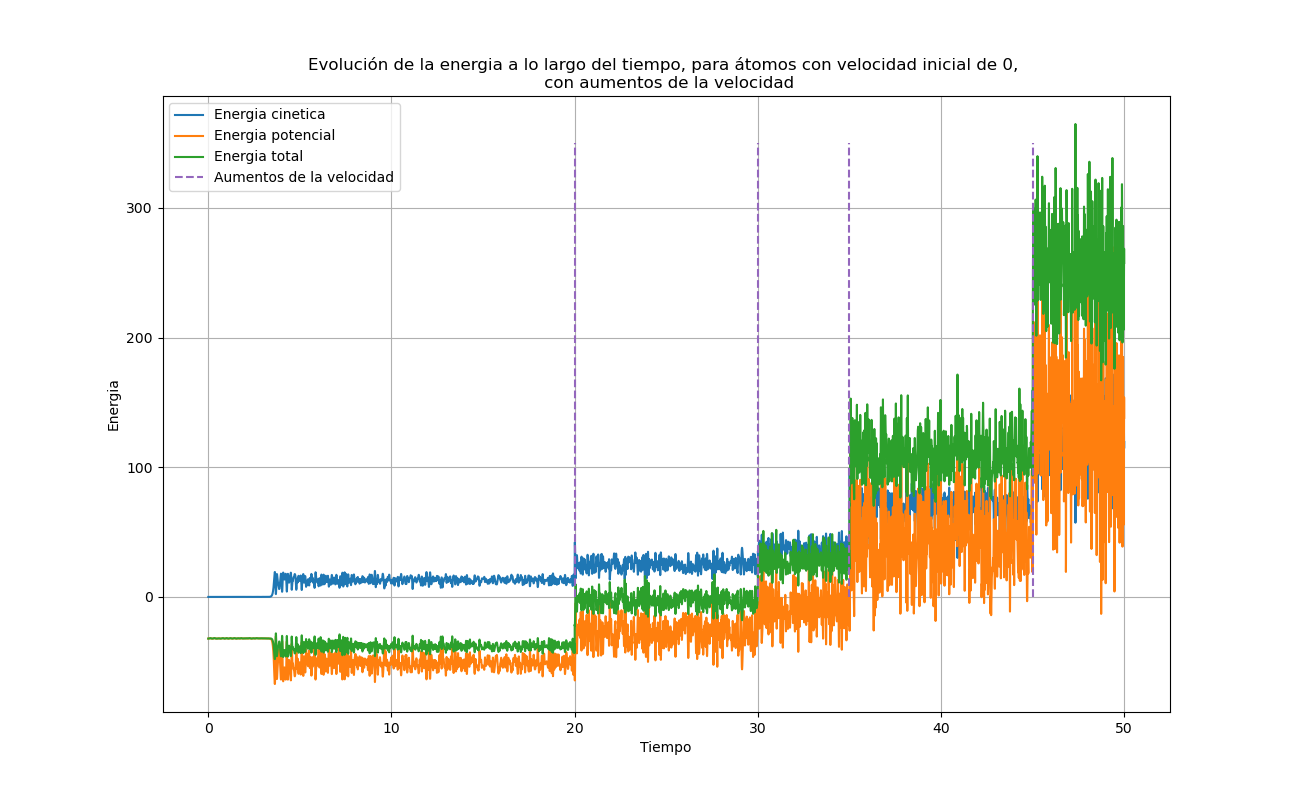
\includegraphics[width=0.9\textwidth]{plots/apartado_6_energia_0.png}
    \caption{Representación de la evolución de las diferentes energías del sistema,
    para un sistema de 16 partículas en una caja de $L=4$, con condiciones iniciales 
    de una red cuadrada y en reposo, aumentando la temperatura en los tiempos 
    $t=20, 30, 35$ y $45$.}
    \label{fig:transicion_fase}
\end{figure}

Sin embargo en esta figura no se observa la transición de fase, para 
ello se emplea el desplazamiento cuadrático medio, representado en la figura 
\ref{fig:desplazamiento_cuadratico_medio_1}. Inicialmente la partícula permanece
en una posición casi fija, pero al aumentar la temperatura, la partícula comienza a
desplazarse más, eso culmina con el tercer aumento de temperatura, donde la partícula
se desplaza de manera considerable, hasta llegar a variaciones abrutas de su posición.
Esto indica la transición de fase del sistema.

\begin{figure}[h!]
    \centering
    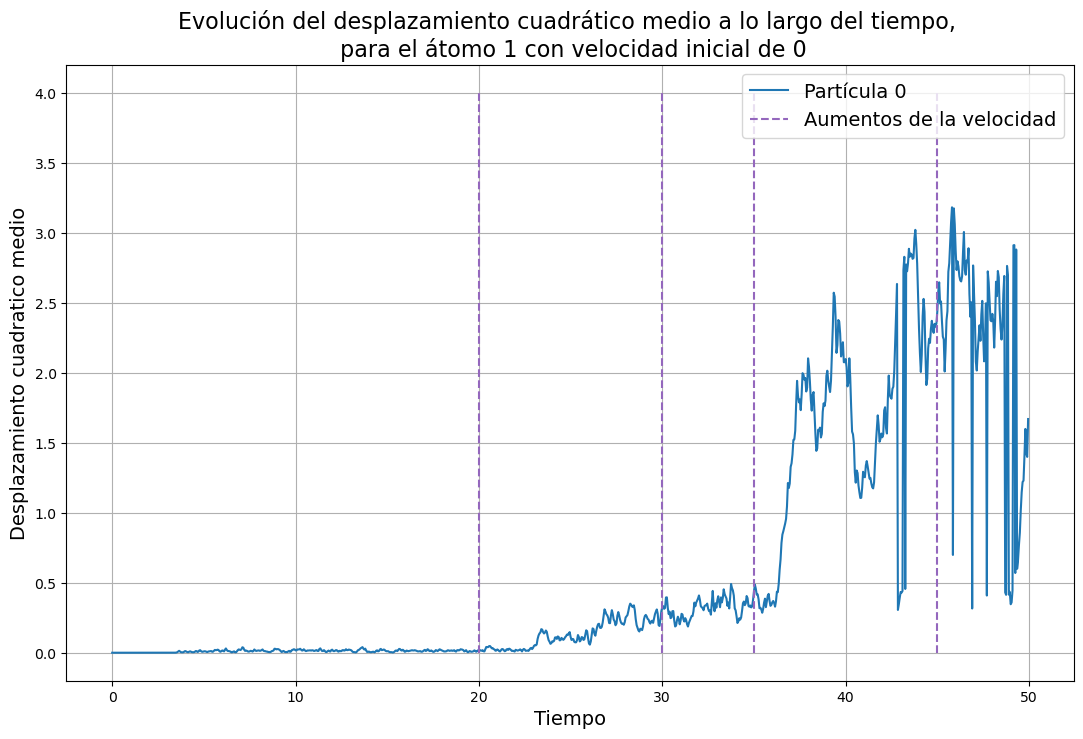
\includegraphics[width=0.9\textwidth]{plots/desplazamiento_1_particula.png}
    \caption{Representación de la evolución desplazamiento cuadrático medio de la 
    partícula 1 del sistema respecto de su posición inicial, para un sistema de 16 
    partículas en una caja de $L=4$, con condiciones iniciales de una red cuadrada 
    y en reposo, aumentando la temperatura en los tiempos $t=20, 30, 35$ y $45$.}
    \label{fig:desplazamiento_cuadratico_medio_1}
\end{figure}

\newpage

\subsection{Temperatura crítica}

El proceso anterior permite para observar el fenómeno de la transición de fase,
sin embargo, para estimar la temperatura crítica, se ha de calentar el sistema más 
lentamente y dejando que el sistema se relaje. 

Para ello se calentará el sistema más lentamente permitiendo que el sistema llegue al 
equilibrio, antes de aumentadar la velocidad en un factor de $1.1$ en los tiempos 
multiplos de $60$, es decir $t=60, 120, 180, ...$. Se ha simulado durante un tiempo 
extensivo $t=600$, con un paso del tiempo $\Delta t = 0.002$, y estudiando el 
desplazamiento cuadrático medio entre 2 partículas cualesquiera, en este
caso se ha elegido la partícula 1 y 7, para obtener la figura 
\ref{fig:energia_temp_crit} para la evolución de las energías del sistema, y la figura
\ref{fig:desplazamiento_cuadratico_medio_1_7} para el desplazamiento cuadrático medio.

\begin{figure}[h!]
    \centering
    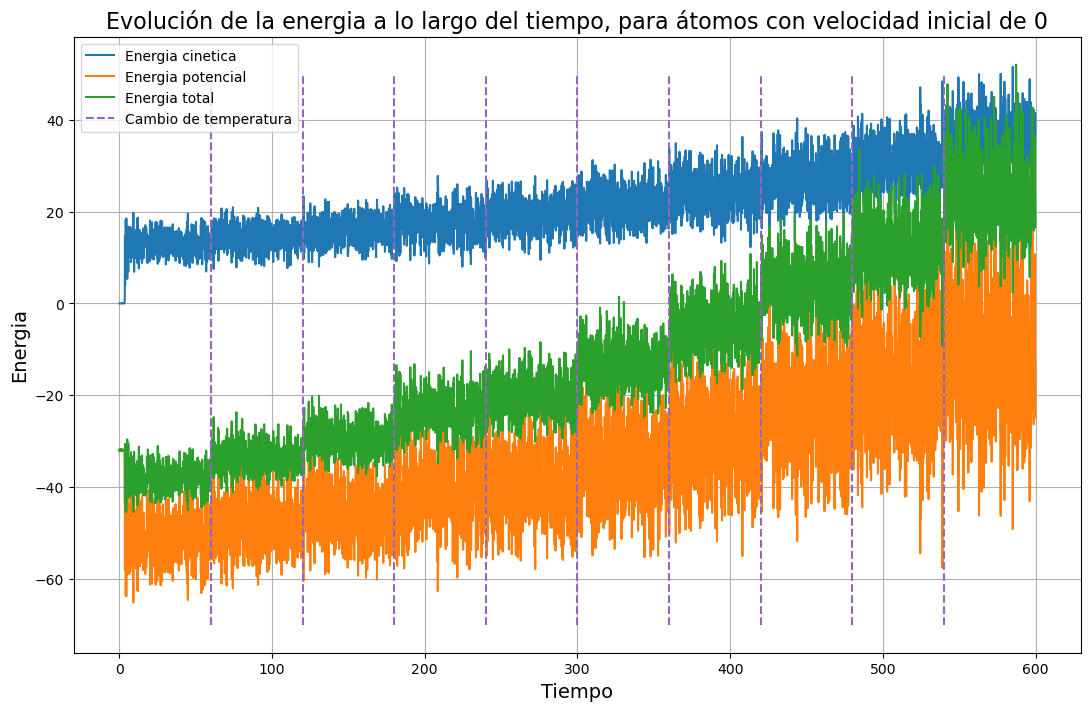
\includegraphics[width=0.9\textwidth]{plots/energia_temp_crit.png}
    \caption{Representación de la evolución de las energías del sistema, para un sistema
    de 16 partículas en una caja de $L=4$, con condiciones iniciales de una red cuadrada 
    y en reposo, aumentando la temperatura en los tiempos $t=60, 120, 180, ...$.}
    \label{fig:energia_temp_crit}
\end{figure}

\begin{figure}[h!]
    \centering
    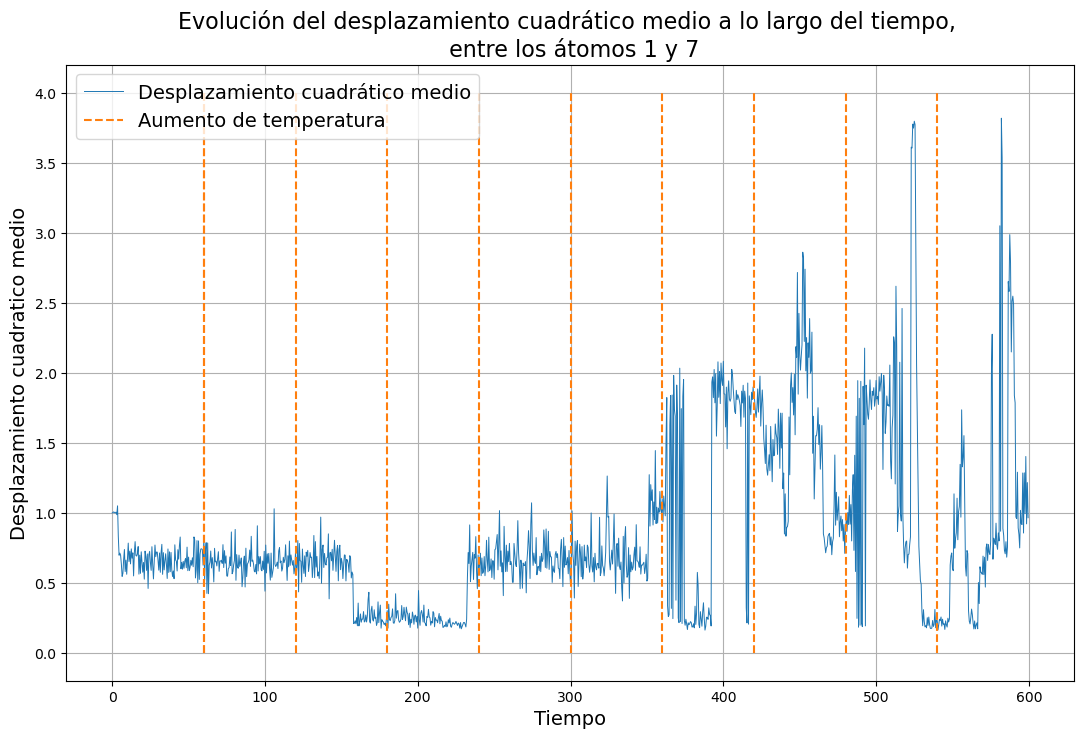
\includegraphics[width=0.9\textwidth]{plots/desplazamiento_temp_crit.png}
    \caption{Representación de la evolución desplazamiento cuadrático medio entre las 
    partículas 1 y 7, para un sistema de 16 partículas en una caja de $L=4$, con condiciones iniciales de una red cuadrada 
    y en reposo, aumentando la temperatura en los tiempos $t=60, 120, 180, ...$.}
    \label{fig:desplazamiento_cuadratico_medio_1_7}
\end{figure}

En cuanto a la evolución de las energías, se observa lo esperado, con cada aumento de 
temperatura, la energía cinética aumenta, causando un aumento tanto en la energía
total como en la potencial.

\newpage

Mientas que para el desplazamiento cuadrático medio, se observa que inicialmente se 
produce una caída en el desplazamiento cuadrático medio, indicando que el sistema ha
alcanzado un estado sólido, la estructura triangular mencionada anteriormente. Con el 
aumento de la temperatura, llega un punto donde disminuye el desplazamiento cuadrático
medio entre dichas partículas, esto se debe a que el sistema ha alcanzado otro estado
de equilibrio, con la misma forma triangular. Este proceso se repite hasta llegar a un
punto donde el desplazamiento cuadrático medio aumenta de manera abrupta, indicando que
se ha alcanzado la temperatura crítica, y el sistema comienza con la transición de fase.

Tras la Transición de fase, el sistema se encuentra en un estado líquido, donde los 
aumento en temperatura aumentan el desplazamiento cuadrático medio, y la energía cinética
del sistema, provocando un movimiento más caótico de las partículas.

\newpage

\subsection{Optimización}

Se estudiará cómo afecta el tamaño del sistema al tiempo de ejecución del programa, 
para distintos parametros de optimización, y distintas máquinas.

Los distintos ordenadores empleados son:
\begin{itemize}
    \item Portatil windows: Intel Core i5-12500H, 16GB RAM, enchufado.
    \item Portatil Macbook Pro M1 (2020), 8GB RAM, desenchufado.
    \item Joel.
\end{itemize}
Y los distintos parametros de optimización empleados son:
\begin{itemize}
    \item Sin optimización.
    \item Optimizando algunas funciones empleadas con \texttt{@jit(nopython=True)}.
    \item Optimizando todas las funciones empleadas con \texttt{@jit(nopython=True)}.
    \item Paralelizando las funciones posibles con \texttt{@jit(nopython=True, parallel=True)}.
    Y empleando distintos números de núcleos.
\end{itemize}

El aumento del tamaño del sistema, es decir el número de partículas se ha realizado
de forma cuadrática ($N = 9, 16, 25, ...$), y la longitud de la caja sería $L = \sqrt{N}$.
De esta manera se simplifica la programación para las condiciones iniciales, procurando
que las partículas estén en una red cuadrada, manteniendo una distancia inicial mínima 
de $1$.

Comenzando con el tiempo de ejecución sin optimizar, se obtiene la figura . Se observa 



Para la simulación con paralelización, se aprecia mucho peor resultado en todos los ordenadores,
indepedientemente del número de núcleos empleados, incluso cuando se compara con el caso sin 
optimizar. Esto indica que la paralelización no es adecuada para este tipo de simulaciones, esto 
puede ser debido a que no existe una gran cantidad de cálculos que se puedan paralelizar, y el 
tiempo de comunicación entre los distintos núcleos o el tiempo empleado en la paralelización
es mayor que el tiempo que se ahorra en los cálculos.
\newpage

\appendix

\section{Tabla de valores}


\newpage

\section{Análisis de errores}


\end{document}
